\chapter{Comparison of Architectures and Loss Functions}
\label{chap:architecture}
In this chapter, I will first introduce some basic types of layers applied in the construction of the DNNs in this thesis. Then I will describe three DNN architectures for Sound Type Classification,  One-Against-All model, SoftmaxWithLoss model and SigmoidCrossEntropy model. At last, I will show the experiment results of these three architectures.

\section{Methods}
In order to accelerate the training process, GPU mode was prefered as the solver\_mode in all of the experiments. 

The performance metric is sensitivity, specificity and balanced accuracy. %TODO:\ref{chapter1 equation}
For a classifier, which classifies all the test sources as positive, it still get a $100\%$ sensitivity. If the amount of true positive points is equal to the amount of true negative points, the accuracy can still reach $50\%$. Considering only the accuracy, the classifier tends to make positive or negative decisions w.r.t the prior of positive and negative sources. That is why  sensitivity, specificity and balanced accuracy were chosen as the performance metrics. Caffe didn't implement a layer for the calculation of sensitivity and specificity. The Accuracy layer produces a metric which can't describe the performance of a classifier well. In order to calculate the sensitivity, I used the python interface in Caffe to extract intermediate outputs of the DNN from the trained model files and calculate these three performance metrics to complete the comparison of different DNN architectures. There are in total 11 classes of sound types, so the performance metrics were calculated for each of these sound types. 

\subsection{Layer Types for Sound Type Classification}
\subsection{Data Layer}
As feature representation for sound type classification, rate maps and AMS features enter the network through data layers. Since both the training dataset and the test dataset are stored in HDF5 files, the data layer type used in this thesis is "HDF5Data" layer.
\subsubsection{Convolutional Layer}
Convolutional layers produce intermediate feature images. As discussed in previous chapter. The adoption of convolutional layers helps in decreasing the weights, which has a positive influence in preventing the overfitting problem. 

\subsubsection{Pooling Layer}
Pooling layers can be seen as a downsampling operation. The input features are convoluted with simple filters, which is usually of size $3\times3$. If the filter operation is to select the maximum value in the neighborhood, such Pooling Layers are called Max Pooling Layers. Pooling layers
add local translation invariance to the network, which improves the generalization of the network\cite{hinton2012improving}. Pooling layers also reduce the amount of parameters and computation in the network, and hence also control the overfitting problem. 
\subsubsection{ReLU Layer}
ReLU layer implements the activation function, defined as:
\begin{align}
f(x) = max(0,x)
\end{align}
In deep neural networks, back propagation through multiple layers with sigmoid activation function may cause the gradient vanish. Compared with sigmoid activation function, ReLU has a constant gradient, as a result, it can be used to reduce likelihood of vanishing gradient. That's why ReLU layers are used in our DNN model.\cite{nair2010rectified}
\subsubsection{Dropout Layer}
Dropout layers randomly switch off part of neurons in the network during training process and increase the output values for the other neurons to normalize. As a result, Dropout layers also help to control overfitting.  Also it
provides a way of implicitly combining many different neural network architectures efficiently\cite{srivastava2014dropout}. The percentage of dropped neurons can be defined as a parameter of dropout layer in Caffe. In this thesis, this parameter was set to $0.5$. 
\subsection{Architectures and Loss Functions}
In this section, three types of DNN architectures for Sound Type Classification will be introduced. Each of these three architecture models are constructed from the layers mentioned in previous section. Also two types of loss functions will be discussed in this section together with corresponding architectures.
\subsubsection{One-Against-All Model}
Sound type classification can be seen as a multi-class classification problem. If we don't consider multi-label classification, a simple model which gives out one scalar output that indicates the class label can be easily constructed in DNN. This model is called One-Against-All model in this thesis. One-Against-All model trains a classifier for 12 classes(11 named classes and a general 'anything else' class). Components of this architecture are shown in Fig.\ref{fig:one-vs-all}. The numbers annotated next to the arrows denote the dimensionalities of output vectors from previous layers.
\begin{figure}[h!]
	\centering 
	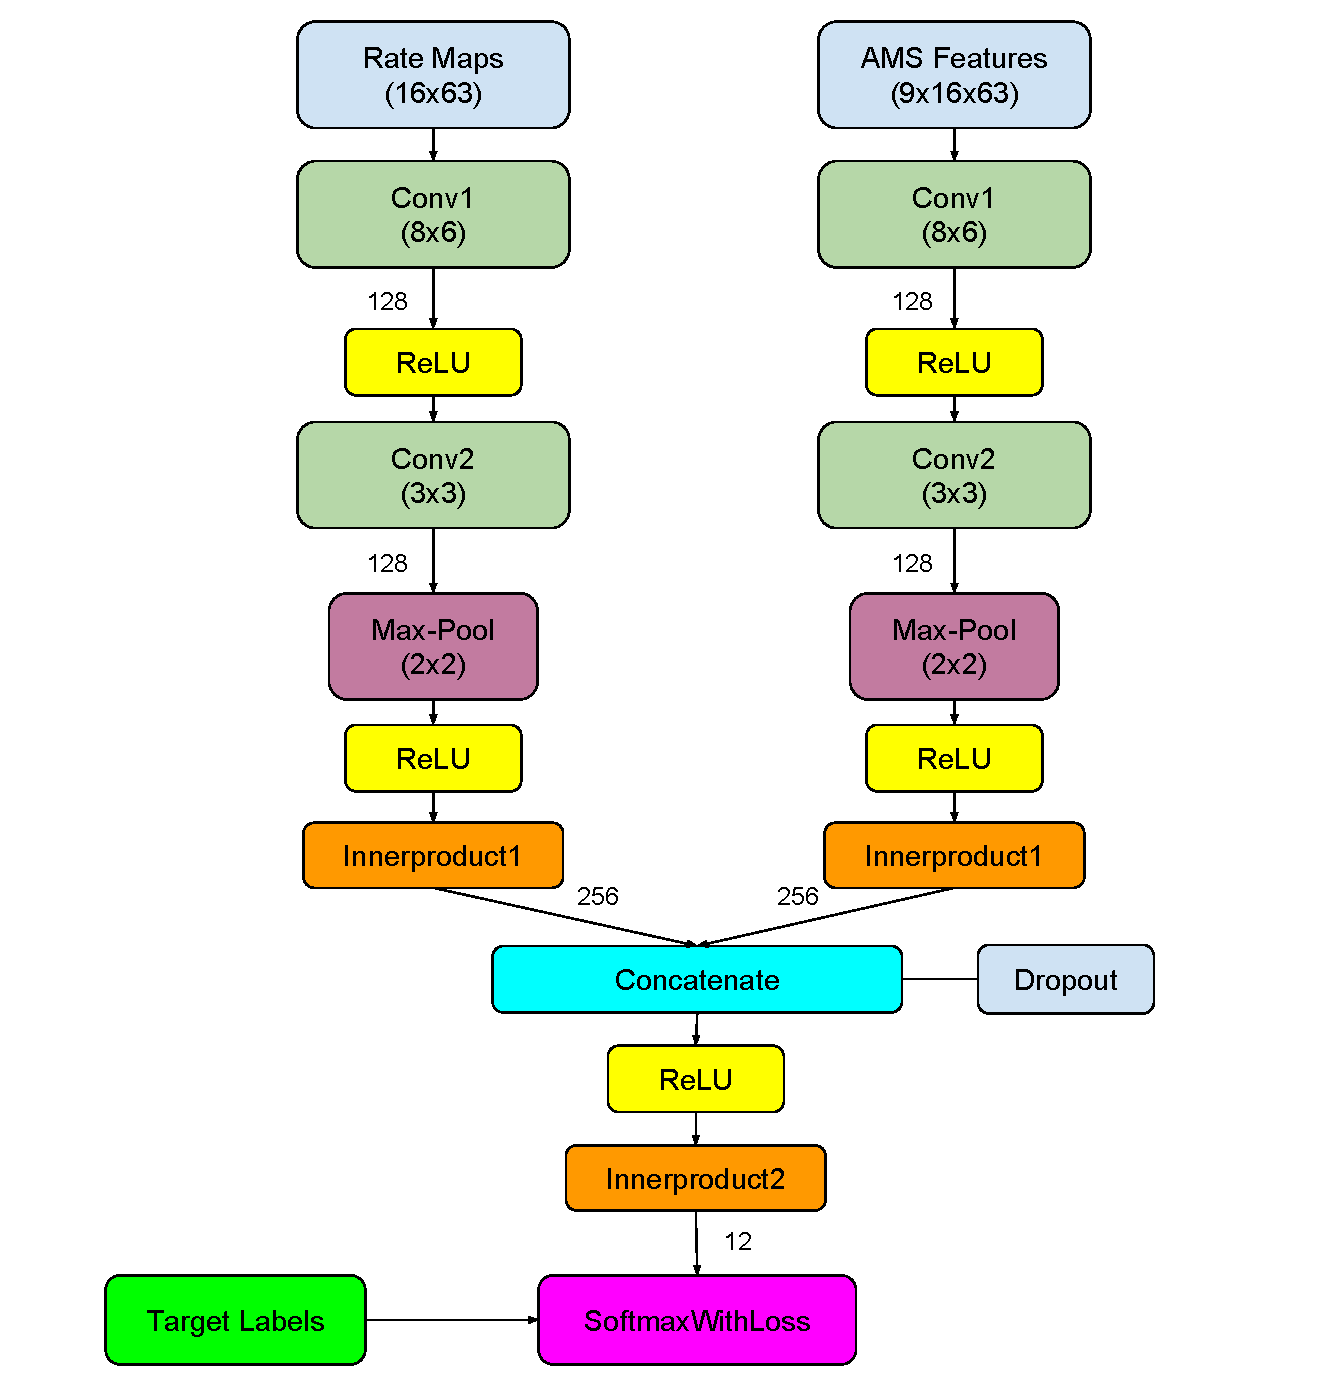
\includegraphics[scale=0.5]{../image/chapter2/Architecture1.pdf}
	\caption{One-Against-All Model architecture visualization}
	\label{fig:one-vs-all}
\end{figure}
One-Against-All model consist of 2 Convolutional layers, 3 ReLU layers, 1 Maxpooling layer, 2 Innerproduct layer,1 Dropout layer and 1 SoftmaxWithLoss Layer. The first Convolutional layer has a kernel size of $8\times 6$ and the second Convolutional layer has a kernel size of $3\times 3$. The output of the second Innerproduct layer is a 12-dimensional vector. The loss layer used in One-Against-All model is SoftmaxWithloss layer. The SoftmaxWithLoss layer computes the multinomial logistic loss of the softmax of its input scores. It takes a batch size of score vectors and true label vectors as inputs. The input scores from previous Innerproduct layer indicates the probability of the assignment to one class label, in other words, the output label would be the index with largest score value in the score vector.
\begin{align}
	\hat{p}_{nk}&=exp(x_{nk})/[\Sigma_{k'}exp(x_{nk'})]\\
	E &= -\frac{1}{N}\Sigma_{n=1}^{N}log(\hat{p}_{nl_n})
\end{align}
Where $\hat{p}_{nk}$ means the probability of input source indexed as $n$ to be classified as class $k$.\\
$x_{nk}$ is the input score of the loss layer. $n$ indicates the input source, $k$ is the index of the score vector from previous layer. The score vector is a 12-dimensional including the score for 'anything else' class.\\
$E$ is the computed cross-entropy classification loss. $l_n$ is the target label of input source indexed as $n$.
\subsubsection{SoftmaxWithLoss Model}
If we consider to build 11 binary classifiers inside one DNN, based on the idea of LASSO binary classifier, the new model can produce a label vector. As a result, this new DNN model can also do the multi-label classification. In this thesis we call this new model SoftmaxWithLoss model. The architecture is shown in Fig.\ref{fig:slicing}. 
\begin{figure}[h!]
	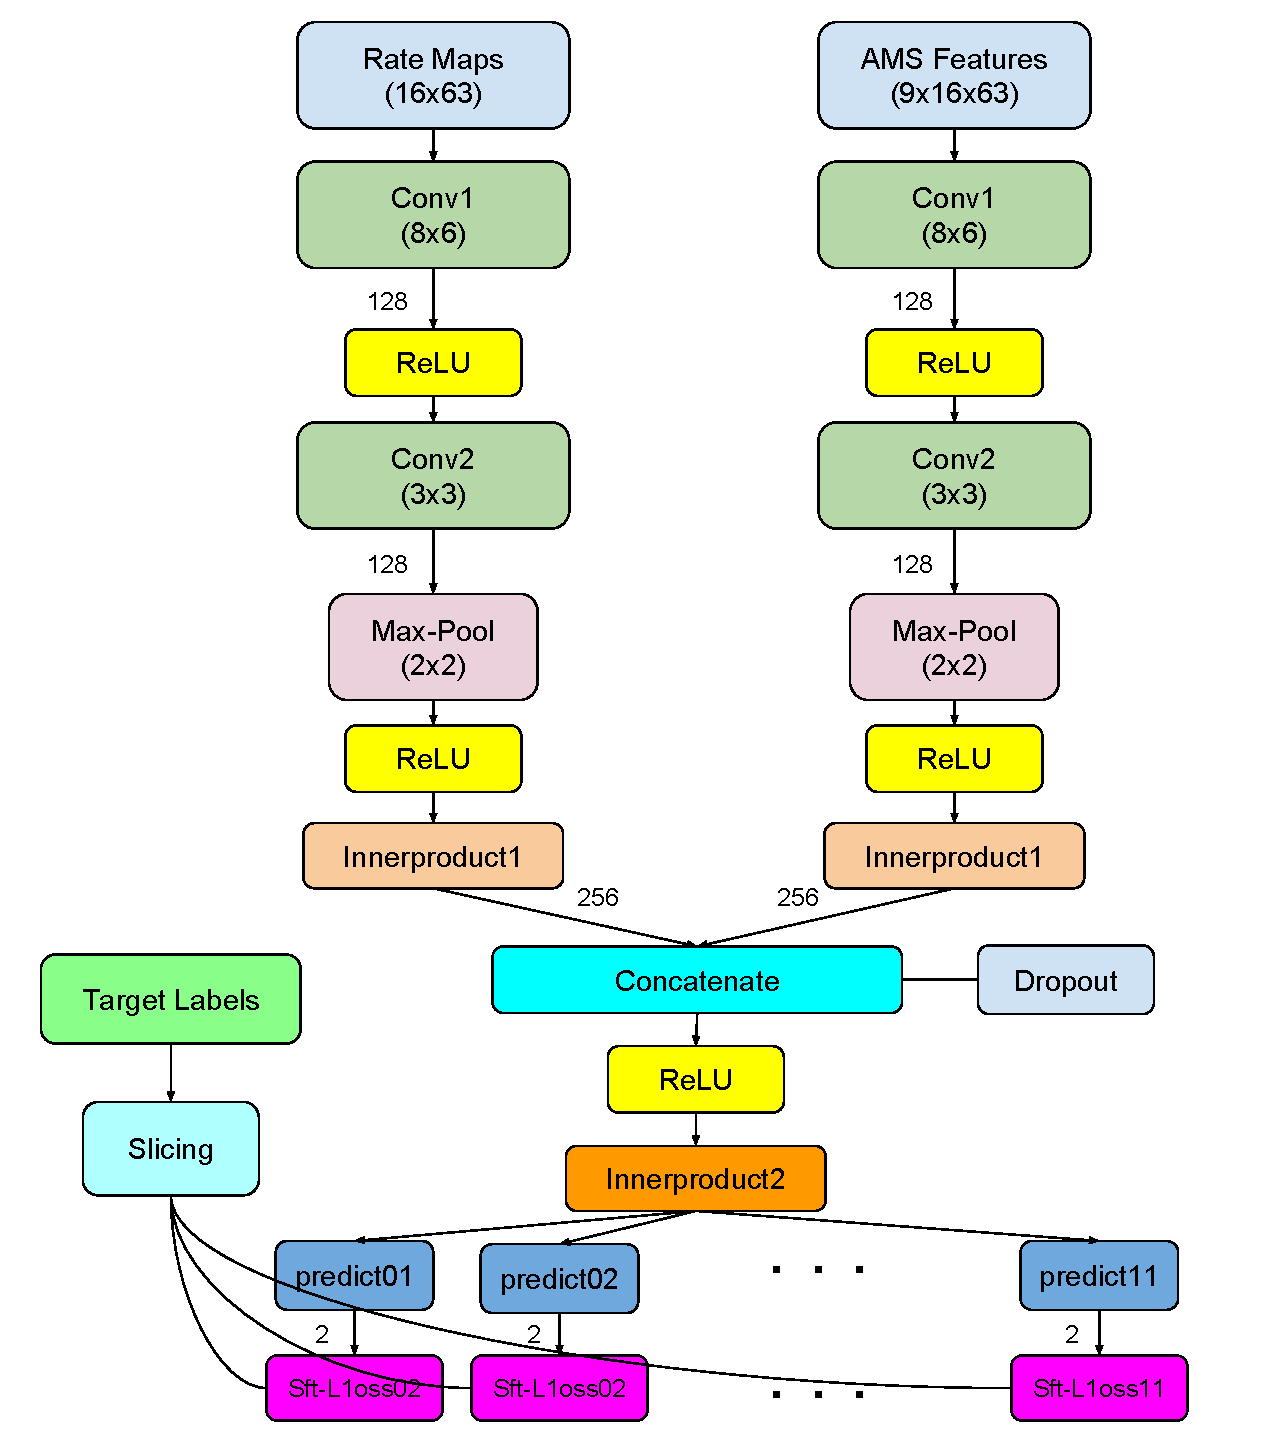
\includegraphics[scale=0.5]{../image/chapter2/Architecture2.pdf}
	\label{fig:slicing}
	\caption{SoftmaxWithLoss Model architecture visualization}
\end{figure}
The basic architecture of the SoftmaxWithLoss model is almost the same as the One-Against-All model. In order to construct a classifier bank inside this network, some changes on the layer that outputs the score vectors should be made. In One-Against-All model, the scores come from an Innerproduct layer, and were passed directly to SoftmaxWithLoss Layer, which calculate an overall loss value as the object function for back propagation. In this SoftmaxWithLoss Model, instead of constructing a 12-dimensional score vector, the output from previous Innerproduct layer, which is in this case a 256-dimensional vector, are further sent to 11 independent Innerproduct layers, the new scores become 2-dimensional vectors and go to 11 independent SoftmaxWithloss layers. The connection between these Innerproduct layers and SoftmaxWithloss layers are one-to-one. At this point, the network is split into 11 branches to train 11 binary classifiers. In each iteration of the model optimization, the model takes a batch size of input sources and split the true labels of the sources into 11 groups w.r.t the label values. The split of true labels are carried out by one Slice layer. These 11 groups of true labels are then passed to these 11 SoftmaxWithLoss layers separately. During the back propagation, the parameters of these Innerproduct layers will be trained to achieve 11 binary classification tasks. 

\subsubsection{SigmoidCrossEntropy Model}
The application of SoftmaxWithLoss layer makes the classification decision in a probabilistic way. If we want to use it for multi-label classification, the only way is to construct a bank of binary classifiers as the SoftmaxWithLoss model. If we consider another decision policy, that sets threshold for the scores and gives out a binary label vector, this also solves the multi-label classification problem. Sigmoid function can maps the scores to probability prediction vectors, each of which only answer the yes-or-no question w.r.t a decided threshold. Inspired by this idea, the SigmoidCrossEntropy Model is constructed using SigmoidCrossEntropy as the loss function. 
\begin{align}
\hat{p}_n &=\sigma(x_n) \\
E &= -1\frac{1}{n}\Sigma_{n=1}^{N}[y_nlog\hat{p}_n+(1-y_n)log(1-\hat{p}_n)]
\end{align}
Where $\hat{p}_{n}$ is the mapped probability from score $x_n$.\\
$y_n$ is the target label of source index as $n$.
$E$ is the computed cross-entropy classification loss. 
The architecture components are almost the same as those in One-Against-All model. Instead of using SoftmaxWithLoss as the loss layer, SigmoidCrossEntropy layer is applied in this model. The architecture visualization is shown in Fig.\ref{fig:sigmoidCE}
\begin{figure}[h!]
	\centering
	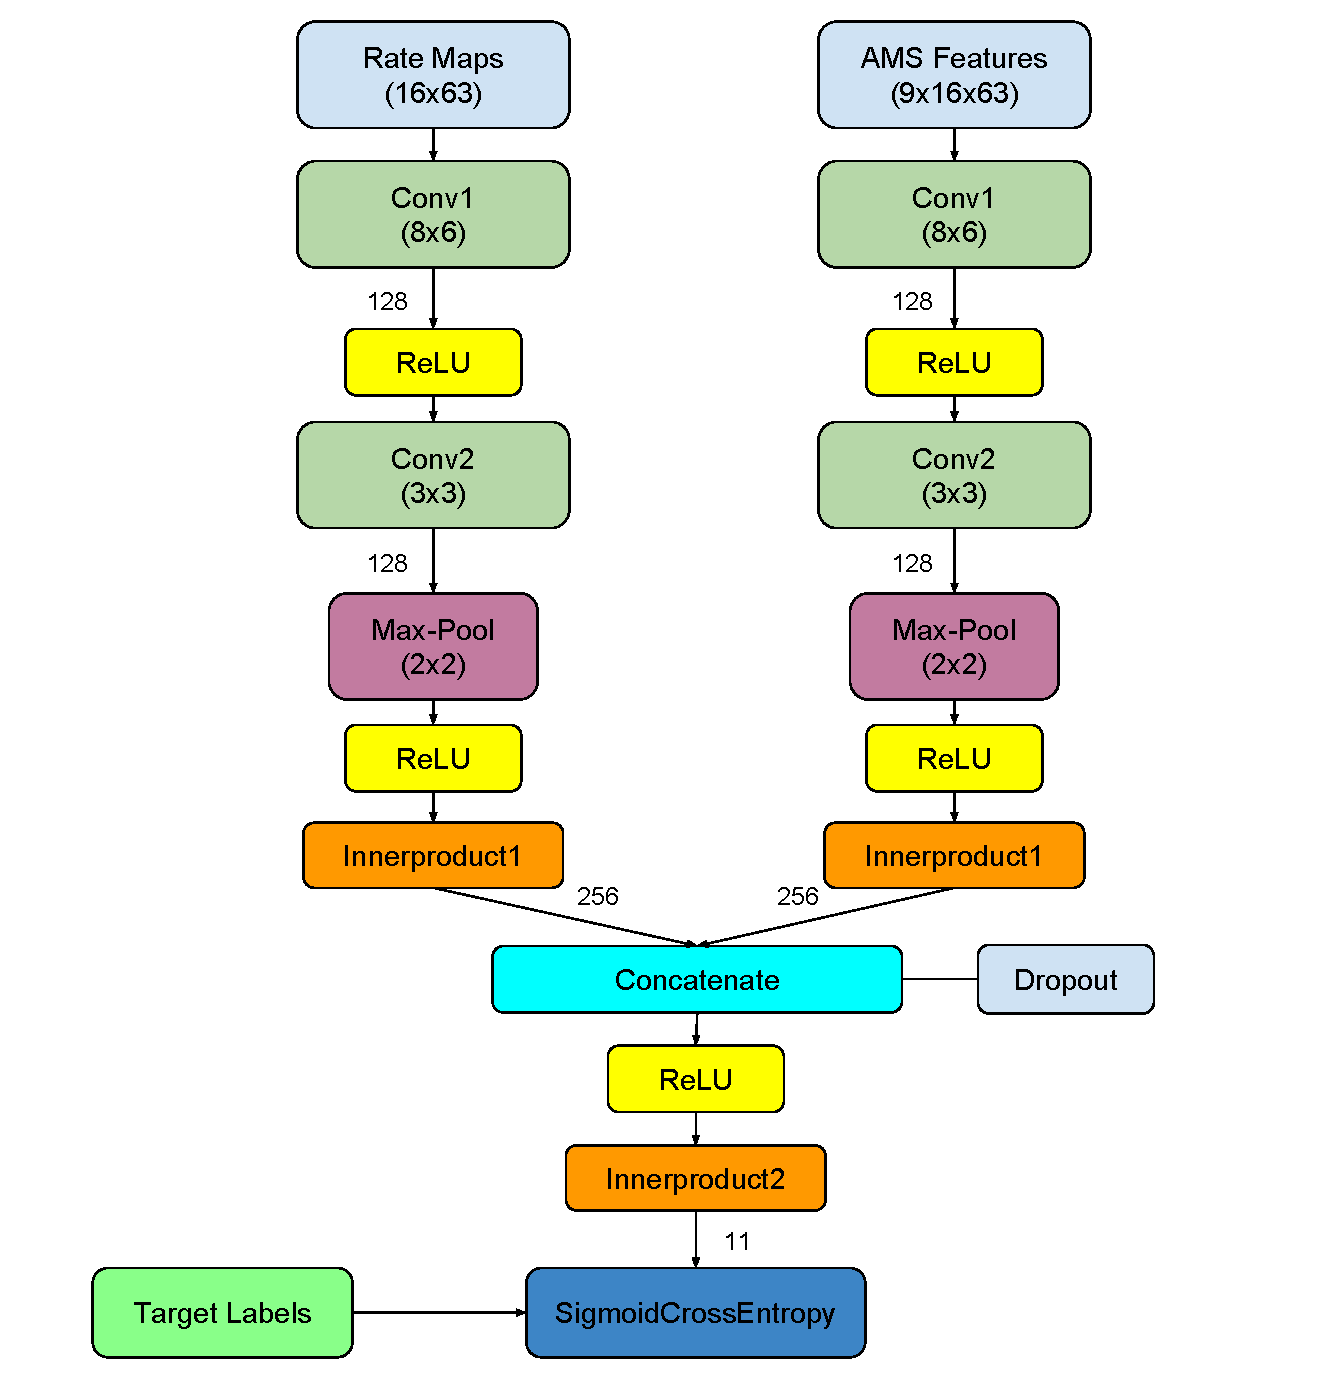
\includegraphics[scale=0.5]{../image/chapter2/Architecture3.pdf}
	\label{fig:sigmoidCE}
	\caption{SigmoidCrossEntropy Model architecture visualization}
\end{figure}
\subsection{Implementation Details}
The training dataset contains  $417888$ feature vectors. For a batch size of $128$, it requires $3265$ iterations to go through all the training data.  So I set the maximum iteration to $100000$ to make sure it converges. The optimization method used in this chapter is Stochastic Gradient Descent(SGD). The initialization strategy for the SGD solvers was the strategy used by Krizhevsky et al. \cite{krizhevsky2012imagenet} in their famously winning CNN entry to the ILSVRC-2012 competition, which has been proved to be a good strategy. The general solver protocol settings are listed in Tab.\ref{tab:solversetting}
\begin{table}[h!]
	\centering
	\begin{tabular}{|c|c|c|c|c|c|c|}
		\hline base\_lr & lr\_policy & gamma & stepsize & momentum & weight\_decay & solver\_mode \\ 
		\hline 1e-4 & step & 0.1 & 30000 & 0.99 & 0.0005  & GPU \\ 
		\hline 
	\end{tabular} 
	\label{tab:solversetting}
	\caption{Optimization Solver Settings}
\end{table}
I also experimented a bit with the Dropout Layer. For each of these three models, I carried out 2 experiments, one with dropout layer, the other without. The dropout ratio were all set to $0.5$.
%(Implementations details enable readers to recover the implementation)\\
%discuss about parameters
\section{Results and Discussion}
\subsection{Learning Curve}
%Also compare with LASSO results
The learning curve of three architectures, displaying the performance metrics during $100000$ iterations, are shown in Fig.\ref{fig:learningcurve}. In each  diagram, the solid lines represent the results of the model with a dropout layer while the dash line without dropout layer. In the legend, 'sens' means sensitivity, 'spec' means specificity and 'bal' means the balanced accuracy.
The learning curve shows that, all of these three models converged before $100000$ iterations. Also for One-Against-All model and SigmoidCrossEntropy model, the difference of the performances seems not so obvious. While in SoftmaxWithLoss model, the adoption of dropout layer contributes a lot for the good performance.
All of these three models get quite high specificity while quite low sensitivity. This means these three models tend to make negative decision. In the rest of this thesis, the main task is to tackle this problem, in order to find a better model with satisfying sensitivity. 

\begin{figure}[h!]
	\centering
	\subfigure[]{
		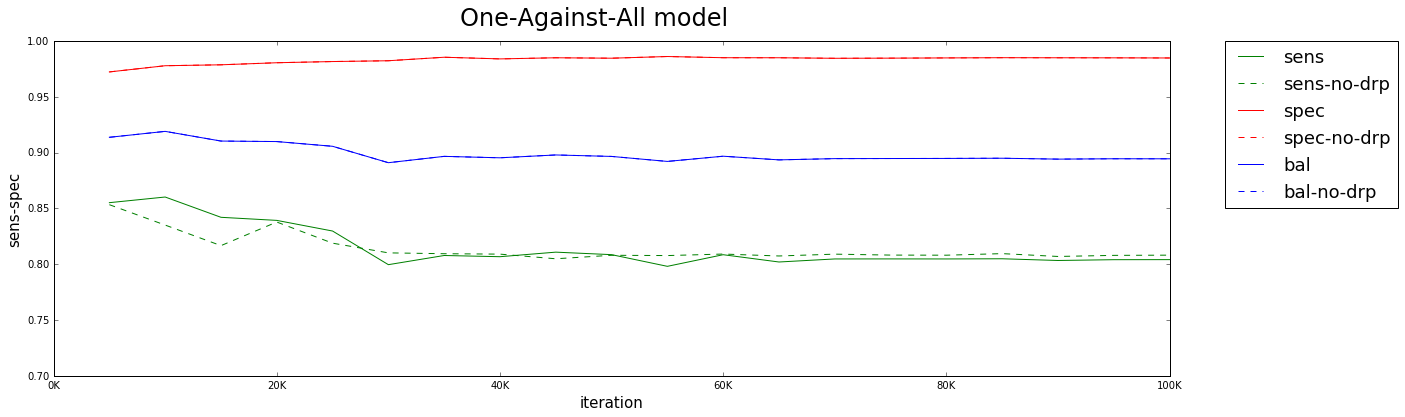
\includegraphics[scale =0.3] {../image/chapter2/one-against-all.png}
		\label{fig:1-vs-all}
	}
	\subfigure[]{
		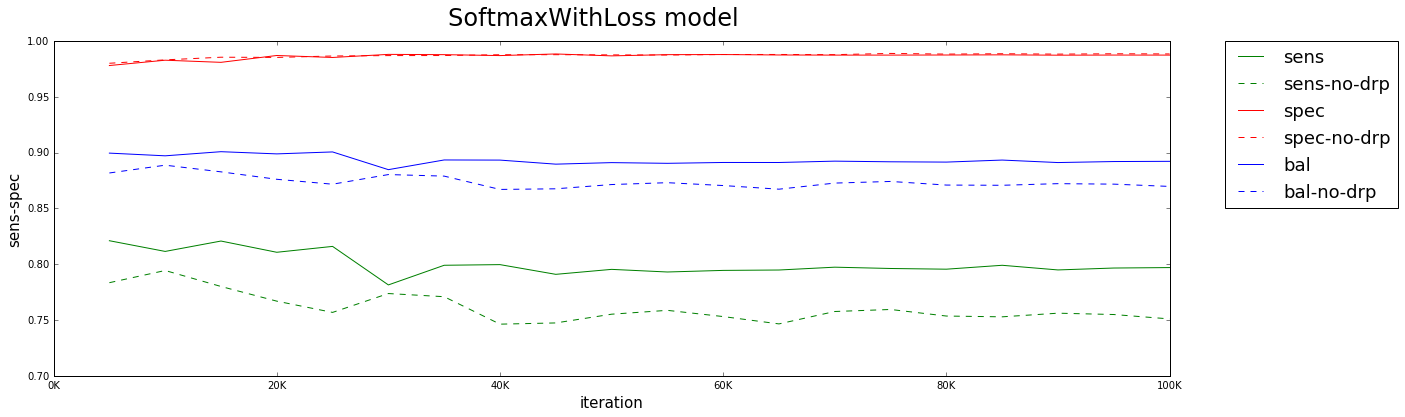
\includegraphics[scale =0.3] {../image/chapter2/SoftmaxWithLoss.png}
		\label{fig:sft}
	}
	\subfigure[]{
		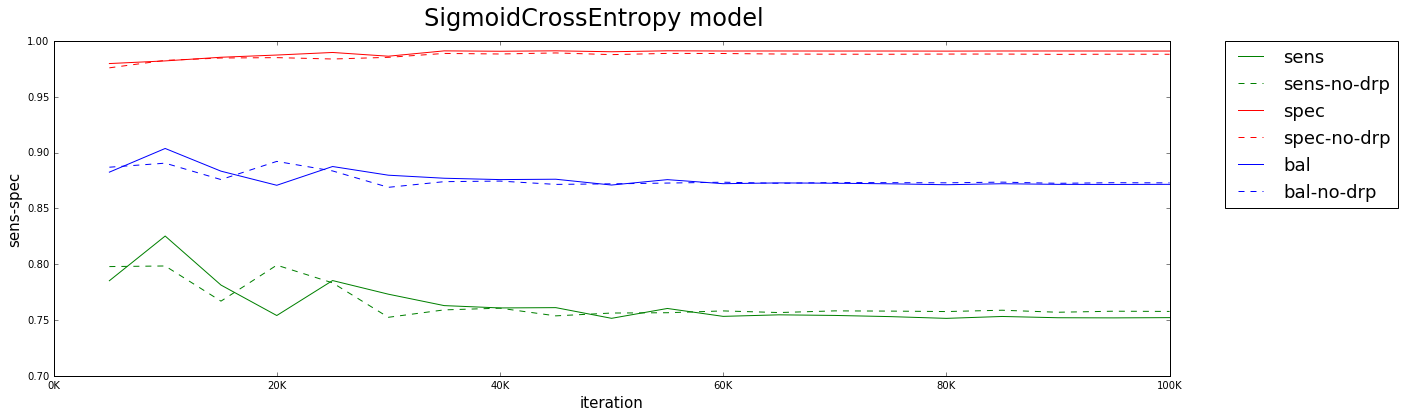
\includegraphics[scale =0.3] {../image/chapter2/SigmoidCrossEntropy.png}
		\label{fig:SCE}
	}
	\caption{Learning curve of 3 architectures}
	\label{fig:learningcurve}
\end{figure}

\subsection{Comparison of Three Architectures}
%The averaged performance metrics over 11 sound type classes of the experiments in this chapter are listed in Tab.\ref{tab:chap2fullresults}
%\begin{table}[h!]
%	\begin{tabular}{|c|c|c|c|}
%		\hline  &  \textbf{balanced accuracy}
%		&  \textbf{sensitivity} 
%		& \textbf{specificity} \\ 
%		\hline \textbf{One-Agains-All}
%		& 0.894 & 0.804 & 0.985 \\ 
%		\hline \textbf{SoftmaxWithLoss}
%		& 0.892 & 0.797 & 0.987 \\ 
%		\hline \textbf{SigmoidCrossEntropy}
%		& 0.872 & 0.752 & 0.991 \\ 
%		\hline 
%	\end{tabular} 
%	\caption{title}
%	\label{tab:chap2fullresults}
%\end{table}
Fig.\ref{fig:spec} shows the specificity accuracy metric for these three architectures. As mentioned above, there is not much difference when comparing these three models with sensitivity metric. However it shows much difference when focusing on the sensitivity metric. As shown in Fig.\ref{fig:sens}, the One-Against-All model shows a pretty good performance. It seems that SigmoidCrossEntropy model does not perform well. Considering the decision policy, SigmoidCrossEntropy model requires a proper setting of threshold. To see how well SigmoidCrossEntropy model can perform, I also plotted the Receiver Operating Characteristic(ROC) curve, see Fig.\ref{fig:rocSCE}. When classifying test sources from type 'alarm', 'crash' and 'engine', the performance has more critical limits than the others. For the other 8 sound types, SigmoidCrossEntropy can still get a good performance if the threshold is properly set. From the sensitivity bar chart Fig.\ref{fig:sens}, 'phone' and 'piano' are also considered as sound types that are difficult to make a classification decision for SoftmaxWithLoss model and One-Against-All model. So in the rest of this thesis, I will focus on SigoidCrossentropy model and do some other improvement based on this model.
\begin{figure}[h!]
	\caption{Specificity of 3 models(with dropout layer)}
	\label{fig:spec}
	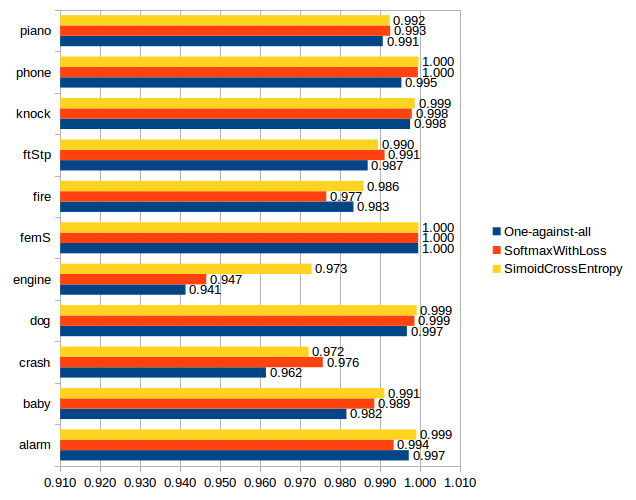
\includegraphics[scale=0.85]{../image/chapter2/Specificity.png} 
\end{figure}


\begin{figure}[h!]
	\caption{Sensitivity of 3 models(with dropout layer)}
	\label{fig:sens}
	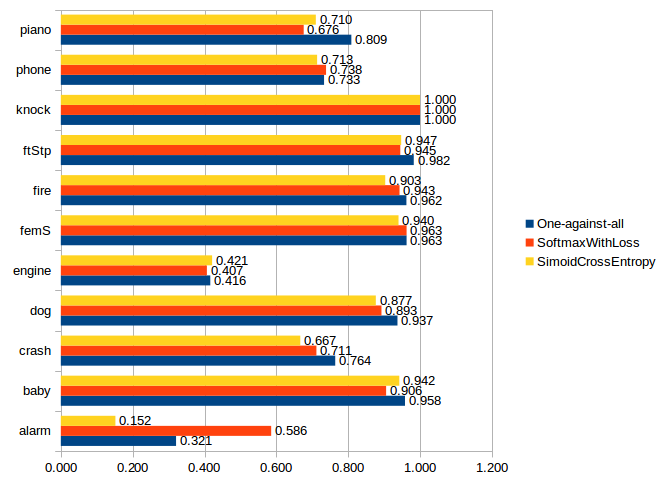
\includegraphics[scale=0.85]{../image/chapter2/Sensitivity.png} 
\end{figure}

\begin{figure}[h!]
	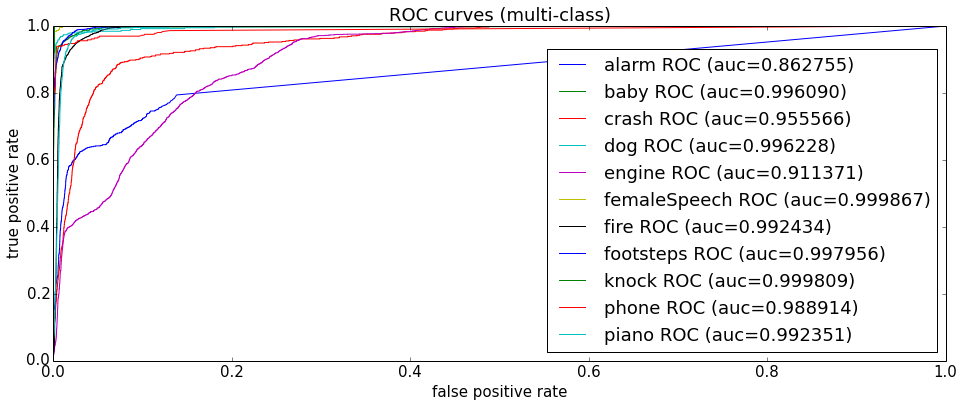
\includegraphics[scale=0.4]{../image/chapter2/rocSCE.png}
	\caption{ROC curve of SigmoidCrossEntropy model(with dropout layer)}
	\label{fig:rocSCE}
\end{figure}
\newpage
To check whether such bad performance comes from the overfitting problem. I also carried out an experiment for SigmoidCrossEntropy model, where I replaced the test dataset with training dataset. The ROC curve of this experiment is shown in Fig.\ref{fig:SCEoverfitting}. 
When testing on the training dataset, SigmoidCrossEntropy model shows a nearly perfect performance. This means the current SigmoidCrossEntropy model meets the overfitting problem. In the rest of this thesis, I will mainly focus on how to deal with this overfitting problem.
\begin{figure}[h!]
	\caption{SigmoidCrossEntropy model tested on training dataset}
	\label{fig:SCEoverfitting}
	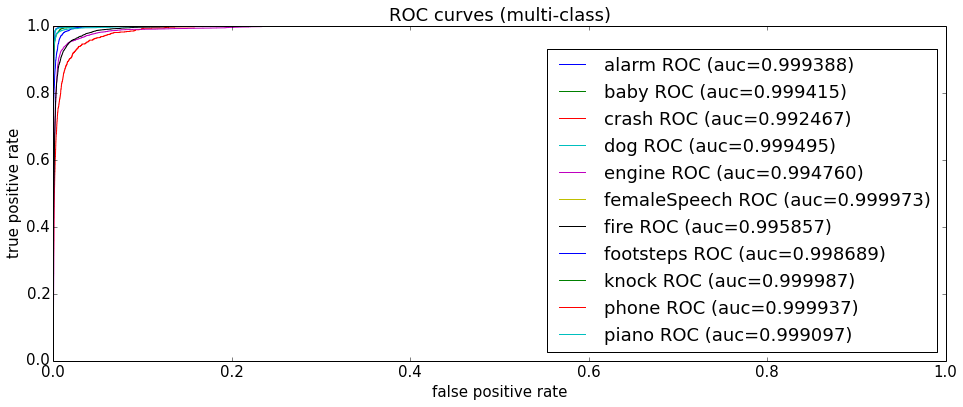
\includegraphics[scale=0.4]{../image/chapter2/SCEoverfitting.png}
\end{figure}